\section{Extensions and Personal Additions}

Beyond the core features, I integrated several extensions to improve the overall quality of the project.

\subsection{Text Rendering Engine (TextRenderer)}
Since the Wayland library did not allow for direct text display, I developed a rendering engine (\texttt{TextRenderer}). It decomposes each character into a pixel matrix (3x5) represented by bitmasks in memory.

\begin{figure}[H]
    \centering
    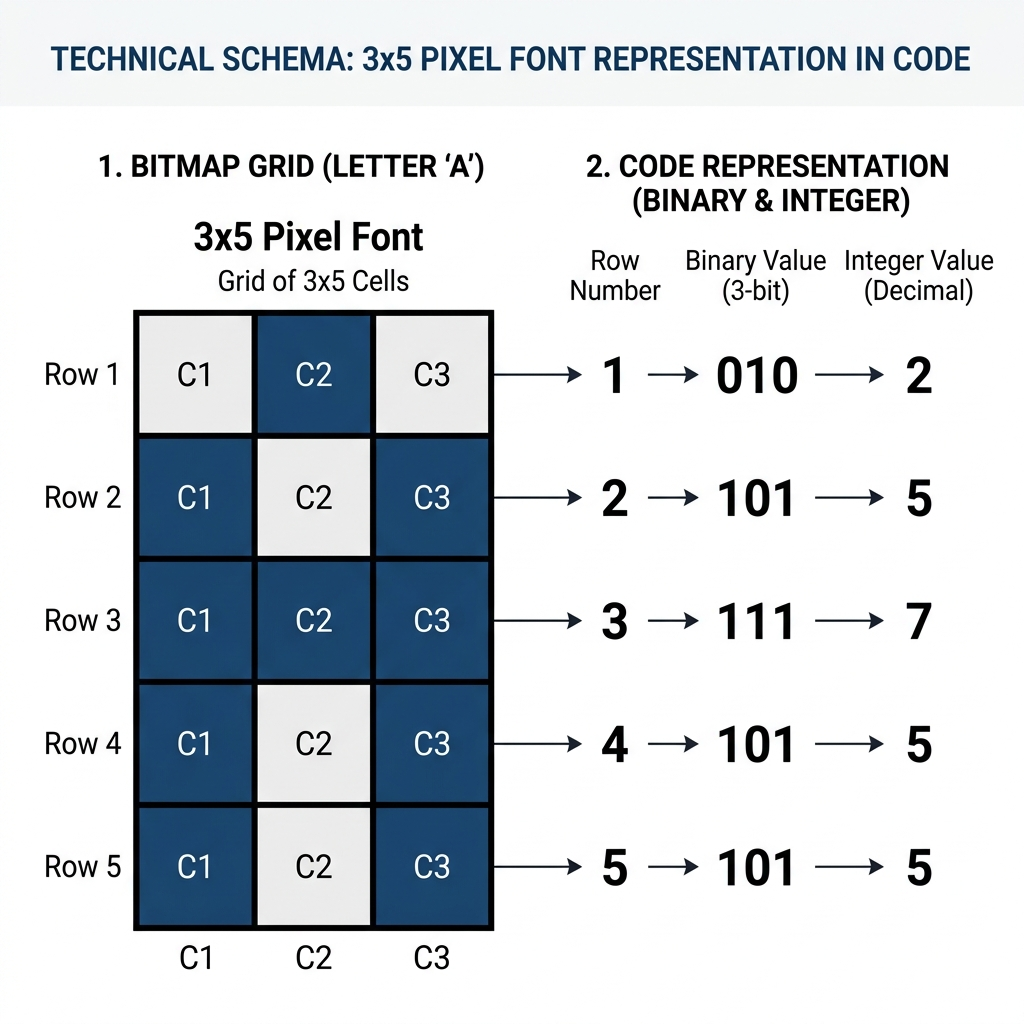
\includegraphics[width=0.45\textwidth]{images/text_renderer_schema.png}
    \caption{Matrix representation of a character in the \texttt{TextRenderer}.}
\end{figure}

\subsection{SmartPlayer: Artificial Intelligence}
Inspired by the INFO8006-1 (Artificial Intelligence) course, I created the \textbf{SmartPlayer} class. It inherits from \texttt{Player} and uses a predictive algorithm to analyze upcoming obstacles and optimize its trajectory in real-time. This mode can be activated by launching the game with the command \texttt{./game -smart}, allowing Thomas to play fully autonomously.

\subsection{Persistent Score Management}
I implemented a \texttt{ScoreManager} that saves records persistently. Scores are now differentiated according to the chosen difficulty level, providing better replayability.

\subsection{Interface and Immersion}
The addition of a smooth main menu, difficulty selection, and a background with a parallax effect contributes to a more immersive user experience.
